%\documentclass[handout]{beamer}
\documentclass{beamer}
%\documentclass[presentation]{beamer}

\usecolortheme{Imperial}
 
\usepackage[utf8]{inputenc}
\usepackage[UKenglish]{babel}
\usepackage{booktabs}
\usepackage{caption}
\usepackage{subcaption}
\usepackage{graphicx}
\usepackage{amsmath}
\usepackage{amsfonts}
\usepackage{amssymb}
\usepackage{epstopdf}

% complying UK date format, i.e. 1 January 2001
%\usepackage{datetime}
%\let\dateUKenglish\relax
%\newdateformat{dateUKenglish}{\THEDAY~\monthname[\THEMONTH] \THEYEAR}

% Imperial College Logo, not to be changed!
\institute{
\includegraphics[height=0.7cm]{Imperial_1_Pantone_solid.eps}}

% -----------------------------------------------------------------------------


%Information to be included in the title page:
\title{Introduction to machine learning and neural networks applied to biological data}

\subtitle{\url{https://bitbucket.org/mfumagal/statistical_inference}}

\author{Matteo Fumagalli}

\date{\today}

\begin{document}
 
\frame{\titlepage}

\begin{frame}
	\frametitle{Intended Learning Outcomes}

	By the end of this session, you will be able to:
	\begin{itemize}
		\item Describe the three key components of a classifier: score function, loss function, optimisation
		\item Identify the elements of a neural networks, including neurons and hyper-parameters
		\item Illustrate the specific layers in a neural network for visual recognition
		\item Appreciate the use of deep learning to solve biological problems
		\item Demonstrate how to implement, train and evaluate a deep neural network in \texttt{python}
	\end{itemize}

\end{frame}

\begin{frame}
	\frametitle{Who is the \textit{deepest learner}?}

	\centering{It's a competition!}

	\begin{columns}
		\column{0.6\textwidth}
		The challenge: predict whether a species is endangered, vulnerable or of least 
		concern from genomic data.
		\column{0.4\textwidth}
		\begin{figure}
                	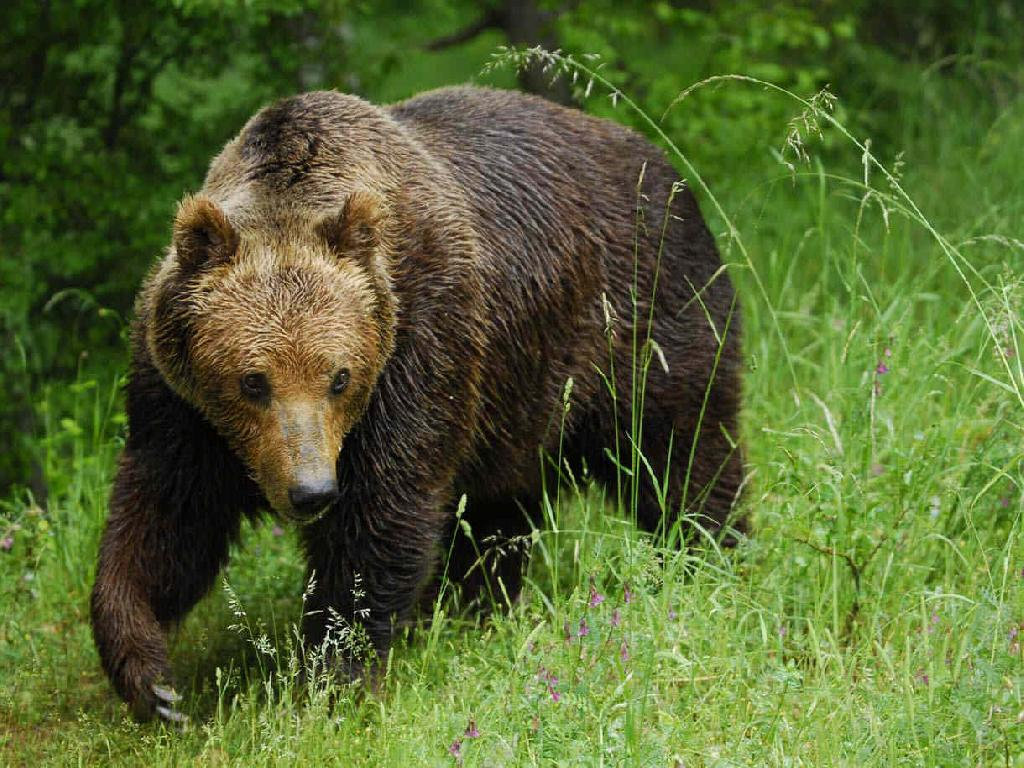
\includegraphics[width=0.8\textwidth]{Pics/ursus.jpg} \\
			\tiny{\textit{Ursus arctos marsicanus}}
        	\end{figure}
	\end{columns}
	
	\vskip 1cm

	The score to beat: 75\% by me.

	The prize: a free drink at the pub.
	
\end{frame}

\begin{frame}
        \frametitle{Evolution of AI}

        \begin{figure}
                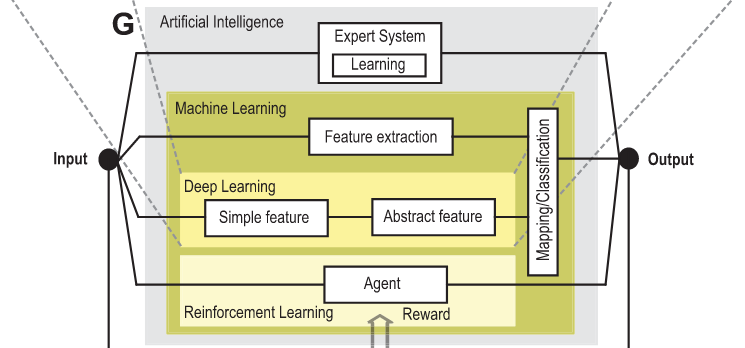
\includegraphics[width=0.9\textwidth]{Pics/evoAI.png}
        \end{figure}

\end{frame}


\section{Image classification}


\begin{frame}
	\frametitle{What do you see?}

	\centering
      	\begin{figure}
               	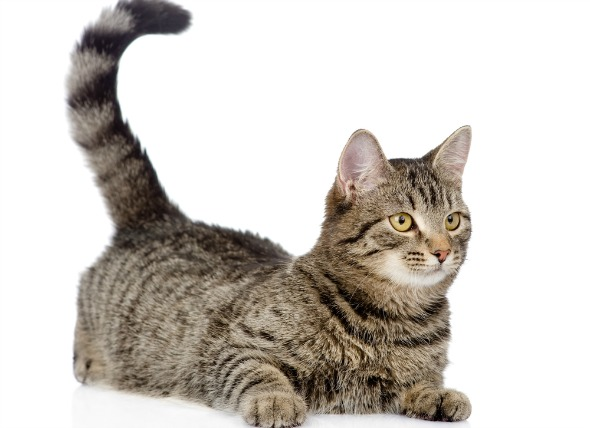
\includegraphics[width=0.75\textwidth]{Pics/cat_generic.jpg}
        \end{figure}

\end{frame}

\begin{frame}
        \frametitle{What does the computer see?}

        \centering
        \begin{figure}
                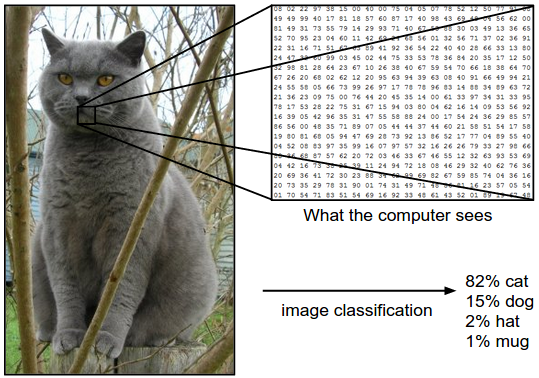
\includegraphics[width=0.7\textwidth]{Pics/cat_computer.png}
        \end{figure}

	Is it THAT difficult?

\end{frame}

\begin{frame}
	\frametitle{Challenges}

	\centering
        \begin{figure}
                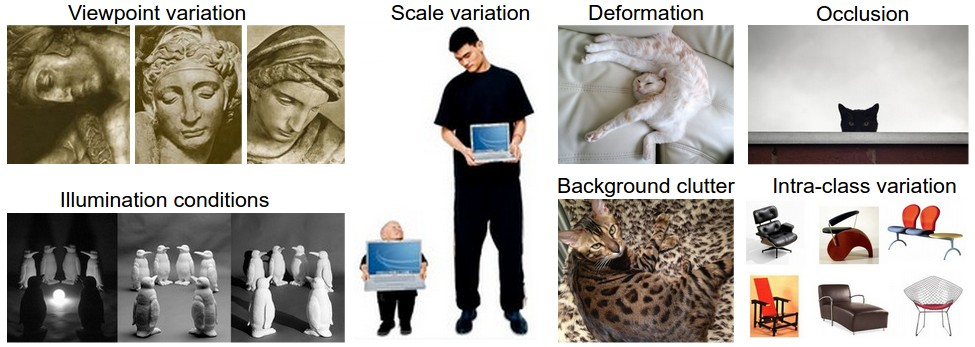
\includegraphics[width=0.9\textwidth]{Pics/challenges.jpeg}
        \end{figure}

	\begin{itemize}
		\item invariant to the cross product of all these variations
		\item retaining sensitivity to the inter-class variations
	\end{itemize}

\end{frame}

\begin{frame}
	\frametitle{Data-driven approach}

	\centering
        \begin{figure}
                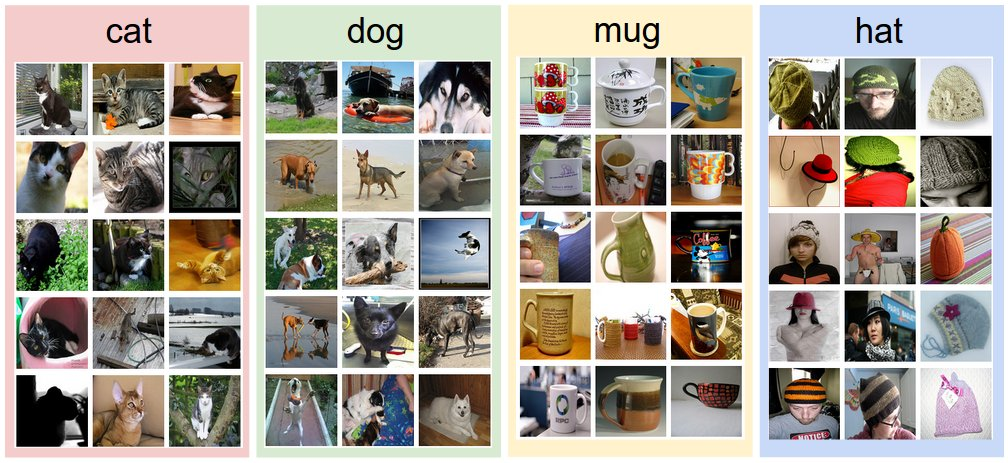
\includegraphics[width=0.7\textwidth]{Pics/trainset.jpg} \\
        \end{figure}

	We need a (large) training dataset of labeled images. 

\end{frame}

\begin{frame}
	\frametitle{Pipeline for image classification}

	\centering
        \begin{figure}
                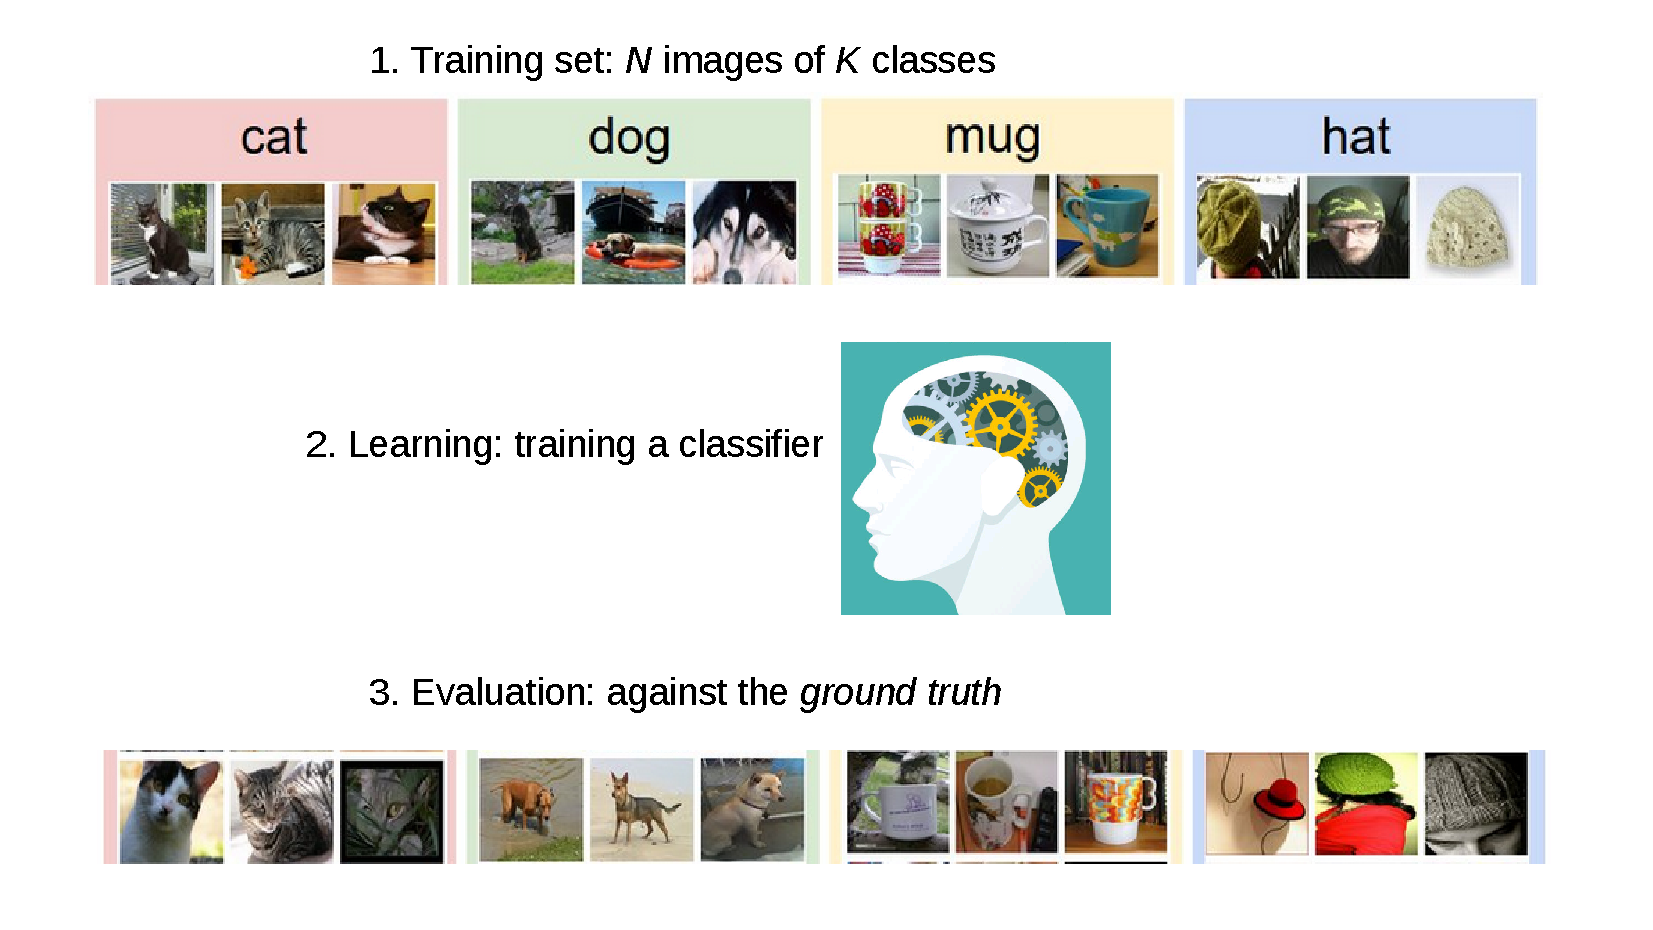
\includegraphics[width=0.9\textwidth]{Pics/pipeline.pdf}
        \end{figure}

\end{frame}

\begin{frame}
	\frametitle{Nearest Neighbour Classifier}

	\centering
        \begin{figure}
                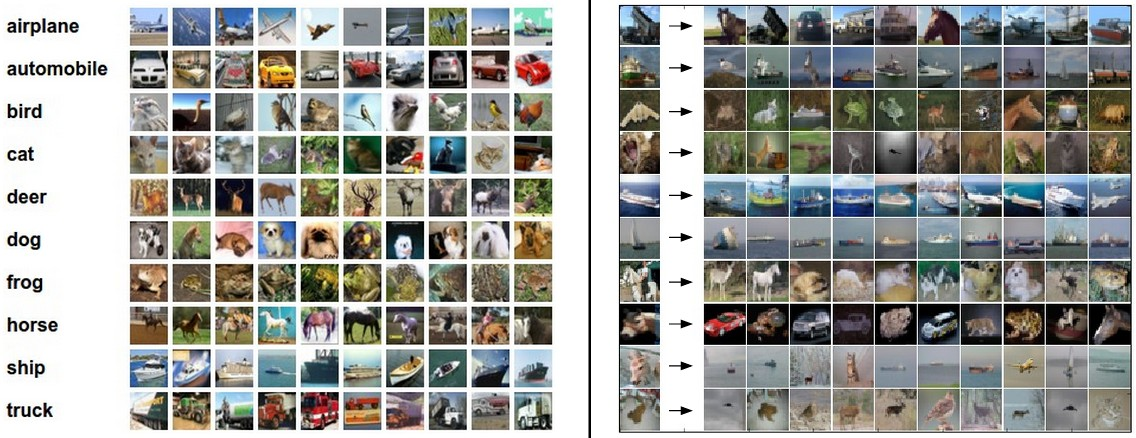
\includegraphics[width=0.9\textwidth]{Pics/nn.jpg} \\
                \caption{CIFAR-10 dataset: 60k tiny images of 10 classes.}
        \end{figure}

	The nearest neighbour classifier will take a test image, \textbf{compare} it to every single one 
	of the training images, and predict the label of the closest training image.

\end{frame}

\begin{frame}
        \frametitle{Nearest Neighbour Classifier}

        \centering
        \begin{figure}
                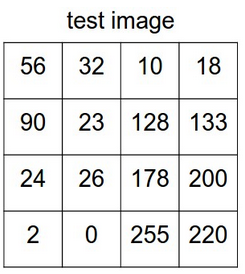
\includegraphics[width=0.4\textwidth]{Pics/nn1.png}
        \end{figure}

\end{frame}

\begin{frame}
        \frametitle{Nearest Neighbour Classifier}

        \centering
        \begin{figure}
                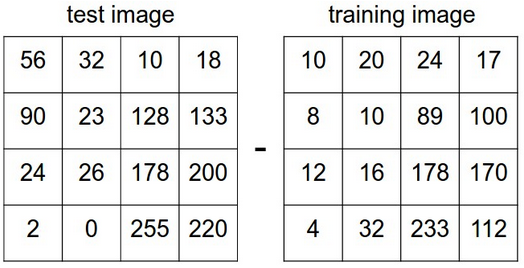
\includegraphics[width=0.7\textwidth]{Pics/nn2.png}
        \end{figure}

\end{frame}

\begin{frame}
        \frametitle{Nearest Neighbour Classifier}

        \centering
        \begin{figure}
                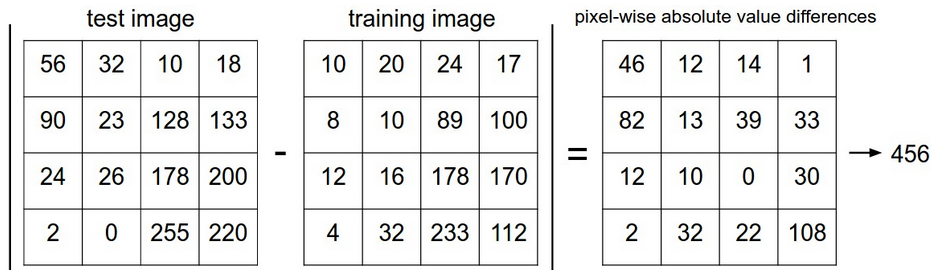
\includegraphics[width=0.8\textwidth]{Pics/nn3.png}
        \end{figure}

\end{frame}

\begin{frame}
	\frametitle{The choice of distance}

	L1 distance: $d_1(I_1,I_2)= \sum_{pixel} |I_1^p - I_2^p|$
	\vskip 0.5cm
	L2 distance: $d_1(I_1,I_2)= \sqrt{ \sum_{pixel} (I_1^p - I_2^p)^2 } $

	\vskip 1cm

	What's their accuracy?\\
	What's human accuracy?\\
	What's state-of-the-art neural networks' accuracy?

\end{frame}

\begin{frame}
	\frametitle{k-Nearest Neighbour Classifier}

	\centering
        \begin{figure}
                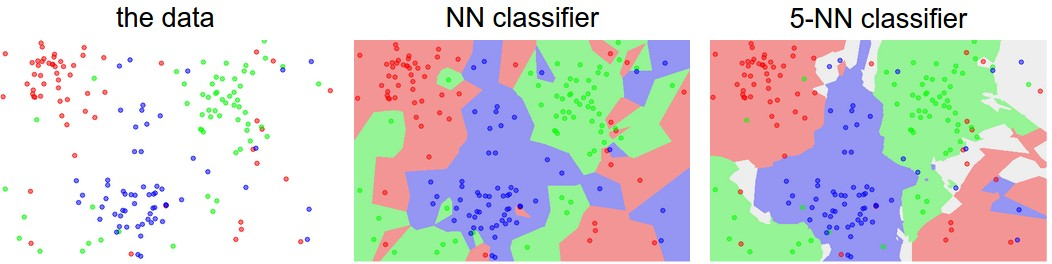
\includegraphics[width=0.9\textwidth]{Pics/knn.jpeg} \\
                \tiny{\caption{An example of the difference between Nearest Neighbor and a 5-Nearest Neighbor classifier, using 2-dimensional points and 3 classes (red, blue, green).}}
        \end{figure}

	What value of \textit{k} should we use? Which distance?

\end{frame}

\begin{frame}
	\frametitle{Hyperparameter tuning}

	\begin{columns}
		\column{0.5\textwidth}
		\begin{figure}
                	
\includegraphics[width=0.6\textwidth]{Pics/engineer.png} \\
        	\end{figure}
		\column{0.5\textwidth}
		The engineer says: "We should try out many different values and see what works best."
	\end{columns}
	\vskip 0.3cm
	\centering
	Agree or disagree?

\end{frame}

\begin{frame}
        \frametitle{Validation test}

        \begin{columns}
                \column{0.5\textwidth}
                \begin{figure}
                        
\includegraphics[width=0.9\textwidth]{Pics/good_engineer.jpg} \\
                \end{figure}
                \column{0.5\textwidth}
                The good engineer says: "Evaluate on the test set only a single time, at the very end."
        \end{columns}

	\begin{itemize}
		\item Split your training set into training set and a validation set. 
		\item Use validation set to tune all hyperparameters. 
		\item At the end run a single time on the test set and report performance.        
	\end{itemize}

\end{frame}

\begin{frame}
	\frametitle{Data splits}

	\begin{figure}
		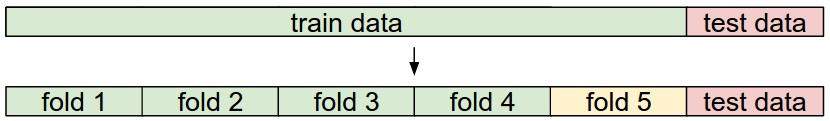
\includegraphics[width=0.9\textwidth]{Pics/crossval.jpeg} \\
		\caption{The training set is split into folds: 1-4 become the training set while 5 is the validation set used to tune the hyperparameters.}
     	\end{figure}

	Where is the Nearest Neighbour classifier spending most of its (computational) time?

\end{frame}

\begin{frame}
	\frametitle{Wrap up}
	
	\begin{itemize}
		\item the problem of image classification: predicting labels for novel test entries
		\item training set vs testing set
		\item a simple Nearest Neighbor classifier requires hyperparameters
		\item validation set to tune hyperparameters
		\item Nearest Neighbor classifier has low accuracy (distances based on raw pixel values!) and is expensive at testing
	\end{itemize}

	Our aim: a solution which gives 90\% accuracy, discards the training set once learning is complete, and evaluates a test image in less than a millisecond!

\end{frame}








\section{Linear classification}

\begin{frame}
	\frametitle{Linear classification}
	
	New approach based on:
	\begin{itemize}
		\item \textbf{score function} to map raw data to class scores
		\item \textbf{loss function} to quantify the agreement between predicted and true labels
	\end{itemize}

\end{frame}

\begin{frame}
	\frametitle{Parameterised mapping from images to label scores}

	Our aim is to define the score function that maps the pixel values of an image to confidence scores for each class.

	\vskip 1cm

	Assuming that:\\
	\centering
	N images, each with dimensionality D, and K distinct classes\\
	$x_i \in R^D$ is image $i$-th with dimensions $D$ and label $y_i$,
	with $i = 1 ... N$ and $y_i \in 1 ... K$
	\vskip 1cm
	then we define a \textbf{score function}: $f: R^D \rightarrow R^K$

\end{frame}

\begin{frame}
        \frametitle{Linear classifier}

	Linear mapping:
	\centering
	$f(x_i; W, b) = W x_i + b$

	\vskip 1cm

	$W$ are called \textbf{weights} and $b$ is the \textbf{bias} vector.
	\vskip 0.5cm
	What are the dimensions of $x_i$, $W$ and $b$?\\

	\pause
	$x_i$ has size [D x 1]\\
	$W$ has size [K x D]\\
	$b$ has size [K x 1]
	

\end{frame}

\begin{frame}
	\frametitle{Linear classifier}

	\centering
	\begin{figure}
		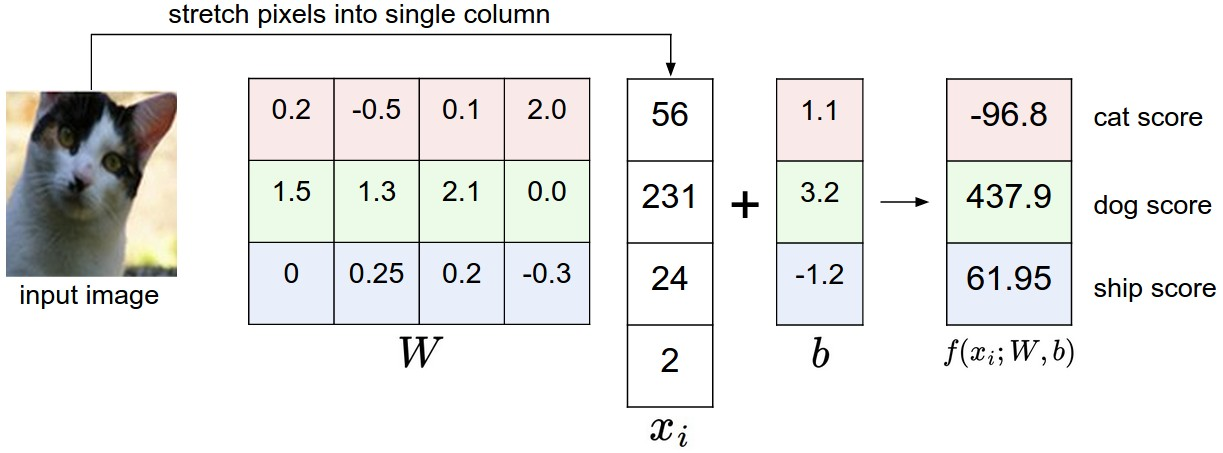
\includegraphics[width=0.9\textwidth]{Pics/imagemap.jpg}
	\end{figure}

\end{frame}


\begin{frame}
	\frametitle{Interpreting a linear classifier (i)}

	\begin{columns}
	
		\column{0.7\textwidth}
        	\begin{figure}
                	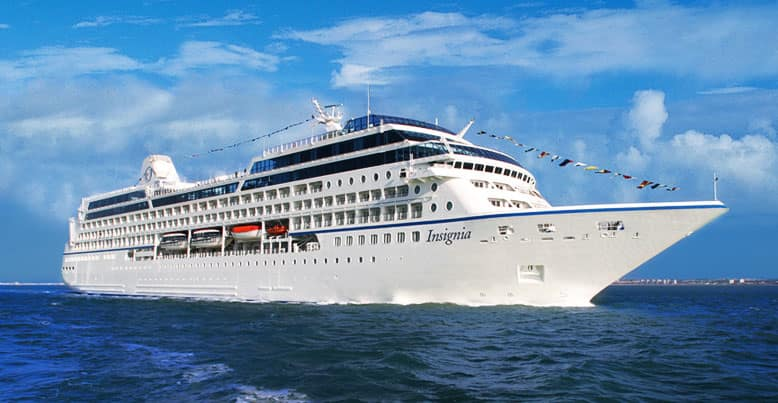
\includegraphics[width=0.8\textwidth]{Pics/ship.jpg}
        	\end{figure}

		\column{0.3\textwidth}
		\begin{figure}
                        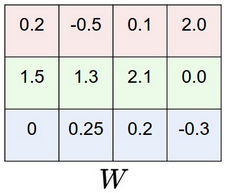
\includegraphics[width=0.8\textwidth]{Pics/W.png}
                \end{figure}
                \begin{figure}
                        
\includegraphics[width=0.6\textwidth]{Pics/like.jpg}
                \end{figure}


		
	\end{columns}

\end{frame}

\begin{frame}
        \frametitle{Interpreting a linear classifier (ii)}

        \begin{columns}
        
                \column{0.6\textwidth}
                \begin{figure}
                        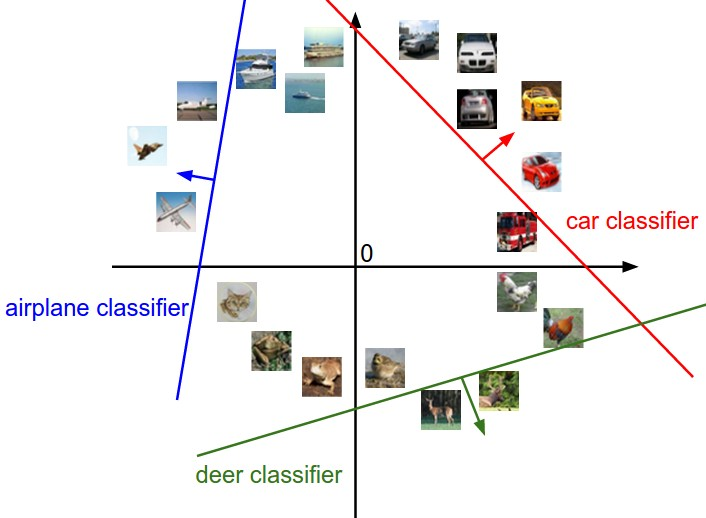
\includegraphics[width=0.9\textwidth]{Pics/pixelspace.jpeg}
                \end{figure}

                \column{0.4\textwidth}
                \begin{figure}
                        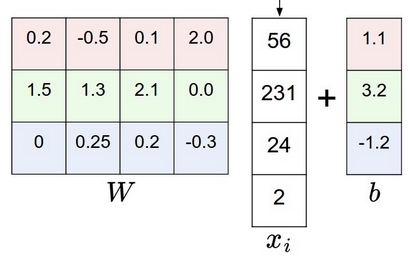
\includegraphics[width=0.9\textwidth]{Pics/Wb.png}
                \end{figure}

        \end{columns}

\end{frame}

\begin{frame}
        \frametitle{Interpreting a linear classifier (iii)}

	Template (or prototype) matching.

        \centering
        \begin{figure}
                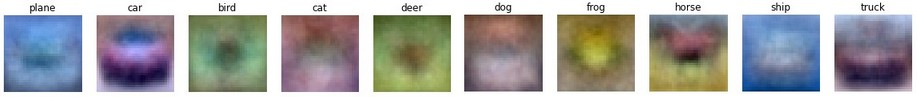
\includegraphics[width=1\textwidth]{Pics/templates.jpg}
        \end{figure}

\end{frame}

\begin{frame}
	\frametitle{Bias trick}

	Our new \textbf{score function}:\\
	$f(x_i; W) = W x_i$
	
	\begin{figure}
      		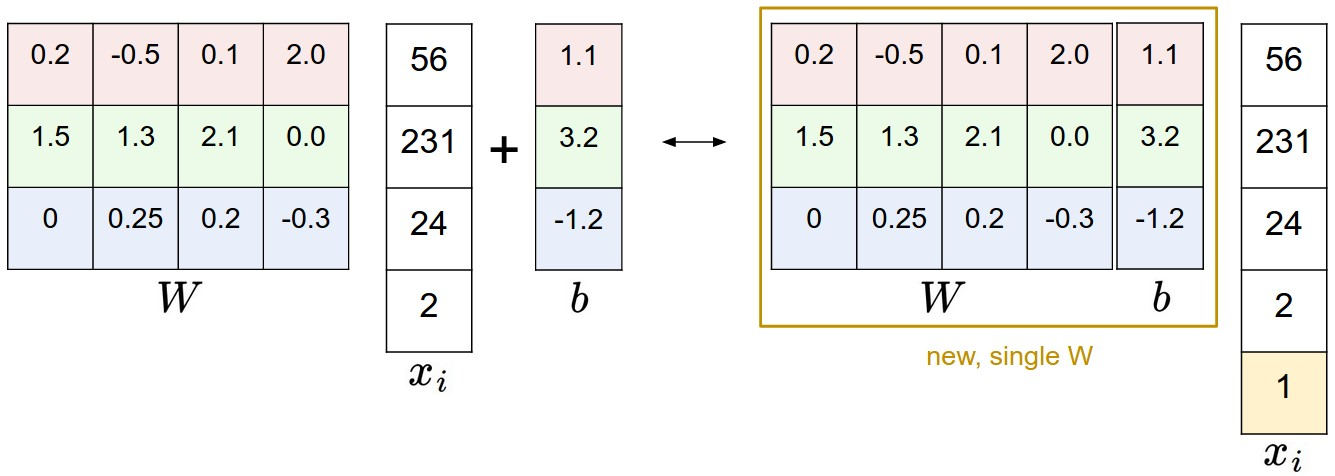
\includegraphics[width=1\textwidth]{Pics/wb.jpeg}
        \end{figure}

\end{frame}

\begin{frame}
	\frametitle{Loss function*}

	\vskip 0.5cm

	To measure our "unhappiness" with predicted outcomes.

	\begin{columns}
		\column{0.8\textwidth}
        	\begin{figure}
                	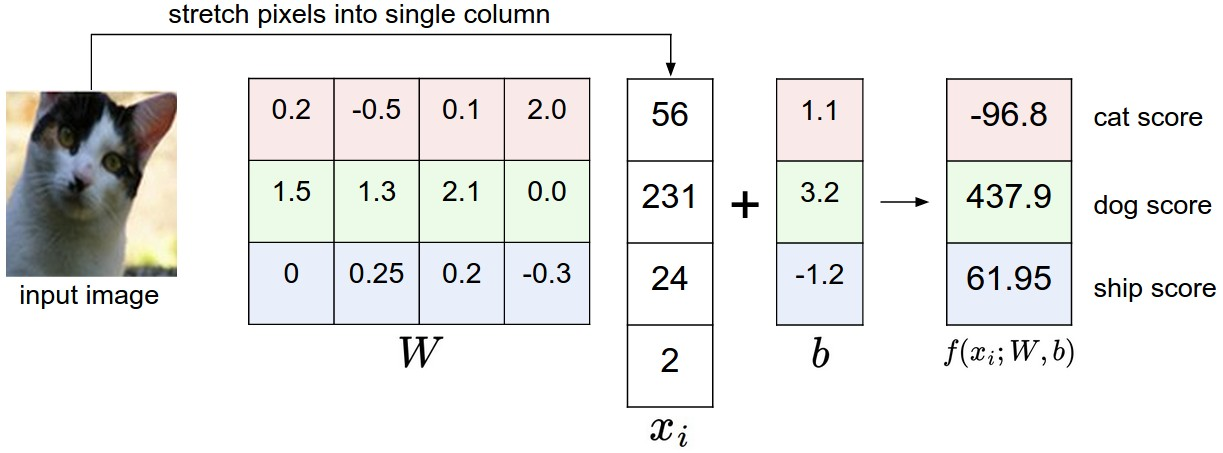
\includegraphics[width=1\textwidth]{Pics/imagemap.jpg}
        	\end{figure}
		\column{0.2\textwidth}
		\pause
                \begin{figure}
                        
\includegraphics[width=0.5\textwidth]{Pics/unhappy.png}
                \end{figure}
	\end{columns}	

	\vskip 1.5cm
	\small{* sometimes called cost function or objective}

\end{frame}

\begin{frame}
	\frametitle{Multiclass Support Vector Machine (SVM) loss}

	The SVM loss is set so that the SVM "wants" the correct class for each image to a have a higher score than the incorrect ones by some fixed margin.

	\begin{equation*}
		L_i = \sum_{j \neq y_i} max (0, s_j-s_{y_i} + \delta)
	\end{equation*}

	Example:\\
	$s=[13,-7,11]$,$y_i=0$,$\delta=10$\\
	$L_i = $ \pause $8$	

\end{frame}

\begin{frame}
        \frametitle{Hinge loss}

	$max(0,-)$ or $max(0,-)^2$

	\centering
	\begin{figure}
      		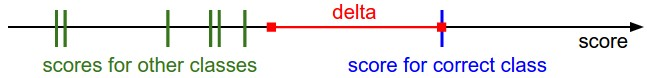
\includegraphics[width=0.9\textwidth]{Pics/margin.jpg}
     	\end{figure}
 
\end{frame}

\begin{frame}
	\frametitle{Regularisation}

	If $W$ correctly classifies each sample, then all $\lambda W$ with $\lambda>1$ will have zero loss.\\
	\vskip 0.2cm
	Which $W$ should we choose?

	\vskip 0.5cm

	\pause
	
	Our new multiclass SVM loss function is:
	\begin{equation*}
                L = \frac{1}{N} \sum_i \sum_{j \neq y_i} [max (0, f(x_i; W)_j - f(x_i; W)_{y_i} + \delta)] + \lambda \sum_k \sum_l W^2_{k,l}
        \end{equation*}
	including one data loss and one regularisation loss term $\lambda R(W)$, specifically L2 penalty.

\end{frame}

\begin{frame}
	\frametitle{Softmax classifier}

	Generalisation of the binary logistic regression classifier to multiple classes.
	\vskip 0.5cm
	Cross-entropy loss function:
	\begin{equation*}
		L_i = -\log ( \frac{ e^{f_{y_i}}} {\sum_j e^{f_j}} )
	\end{equation*}
	
\end{frame}

\begin{frame}
	\frametitle{Probabilistic interpretation of Softmax scores}

	\begin{equation*}
      		P(y_i | x_i; W) = \frac{ e^{f_{y_i}}} {\sum_j e^{f_j}}
        \end{equation*}

	Likelihood or Bayesian?

\end{frame}

\begin{frame}
	\frametitle{SVM vs. Softmax classifier}

	\centering
        \begin{figure}
                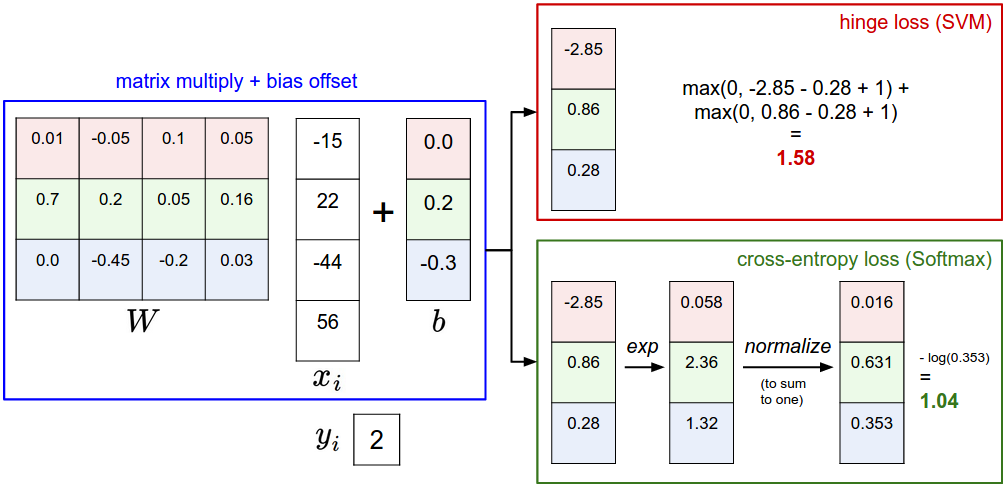
\includegraphics[width=0.9\textwidth]{Pics/svmvssoftmax.png}
        \end{figure}

\end{frame}

\begin{frame}
	\frametitle{Wrap up}

	\begin{itemize}
		\item A score function maps image pixels to class scores (using
		 a linear function that depends on W and b).
		\item Once we learning is done, we can discard the training data
		and prediction is fast.
		\item A loss function (e.g. SVM and Softmax) measures how 
		compatible a given set of parameters is with respect to the 
		ground truth labels in the training dataset. 
	\end{itemize}

	How do we determine (optimise) the parameters that give the lowest loss?

\end{frame}






\section{Optimisation}

\begin{frame}
	\frametitle{Key components for image classification}

	\begin{enumerate}
		\item score function
		\item loss function
		\item optimisation
	\end{enumerate}

	Optimisation is the process of finding the set of parameters $W$ that 
	minimise the loss function $L$.

\end{frame}

\begin{frame}
	\frametitle{Visualising the loss function}

	\vskip 0.5cm
	If $W_0$ random starting point, $W_1$ random direction, then compute 
	$L(W_0 + a W_1)$ for different values of $a$.

	\centering
        \begin{figure}
                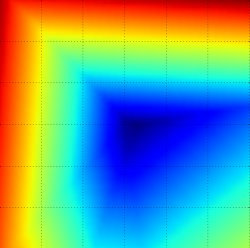
\includegraphics[width=0.35\textwidth]{Pics/svm_one.jpg}
        \end{figure}
	
	\small{(averaged across all images, $x_i$)}

\end{frame}

\begin{frame}
	\frametitle{Optimisation}

	\begin{columns}
		
		\column{0.3\textwidth}
		\begin{figure}
	                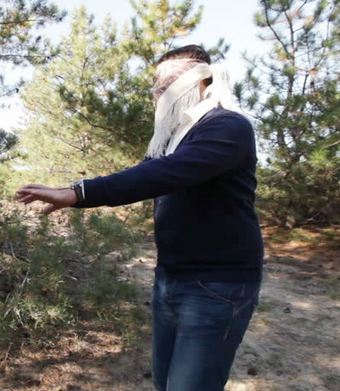
\includegraphics[width=0.8\textwidth]{Pics/hiker.png}
        	\end{figure}
		\column{0.7\textwidth}
		\begin{itemize}
			\item Random search
			\item Random local search
			\item Gradient descent (numerical or analytical)
		\end{itemize}

	\end{columns}

	\vskip 1cm
	\begin{equation*}
		\frac{df(x)}{dx} = \lim_{h \rightarrow 0} \frac{f(x+h)-f(x)}{h}
	\end{equation*}

\end{frame}

\begin{frame}
	\frametitle{Hyperparameters}

	\begin{columns}
		\column{0.5\textwidth}
		\textbf{Step size} or learning rate
		\centering
		\begin{figure}
                	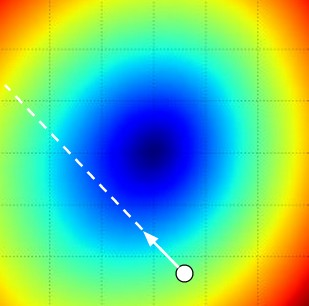
\includegraphics[width=0.8\textwidth]{Pics/stepsize.jpg}
        	\end{figure}
		\column{0.5\textwidth}
		\textbf{Batch size}:\\
		Compute the gradient over batches (e.g. 32, 64, 128...) of the 
		training data.
	\end{columns}

\end{frame}

\begin{frame}
	\frametitle{Backpropagation}

	\vskip 0.3cm
	We can compute the gradient analytically using the chain rule.

	\vskip 0.5cm

	\centering
	$f(x,y,z)=(x+y)z$\\
	$q=x+y$ and $f=qz$\\
	$\frac{df}{dx}=\frac{df}{dq}\frac{dq}{dx}$

        \begin{figure}
                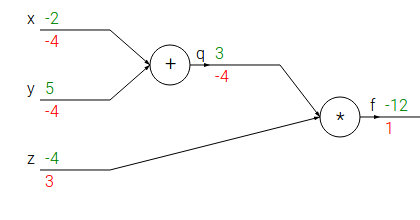
\includegraphics[width=0.6\textwidth]{Pics/backpropagation}
        \end{figure}

\end{frame}


\begin{frame}
	\frametitle{Wrap up}

	\centering
	\begin{figure}
        	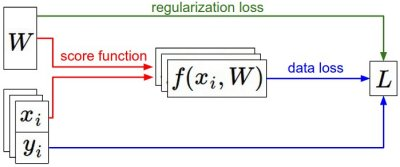
\includegraphics[width=0.7\textwidth]{Pics/dataflow.jpeg}
      	\end{figure}

	The 3 elements: score function, loss function, optimisation.

	Next: let's put them all together in a neural network.

\end{frame}


















\section{Neural networks}

\begin{frame}
	\frametitle{Neurons}

	\centering
        \begin{figure}
                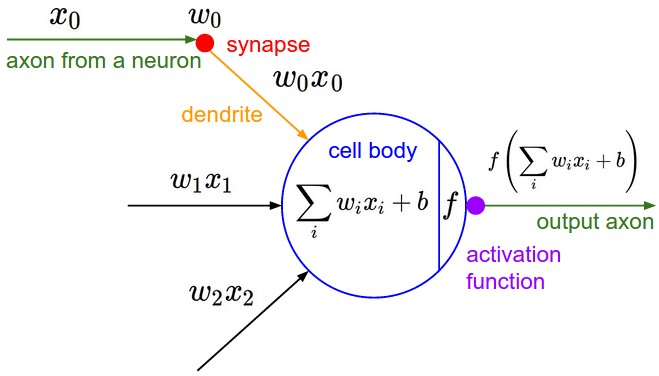
\includegraphics[width=0.7\textwidth]{Pics/neuron_model}
        \end{figure}

\end{frame}

\begin{frame}
	\frametitle{Activation functions}
	
	\centering{It defines the \textit{firing rate}}

	\begin{columns}
		\column{0.5\textwidth}
		\begin{figure}
                	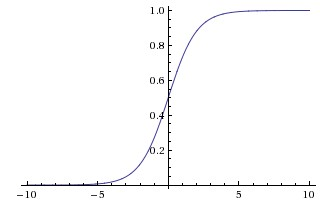
\includegraphics[width=0.7\textwidth]{Pics/sigmoid}\\
			\small{Sigmoid non-linearity squashes real numbers to range between $[0,1]$}
        	\end{figure}
		\column{0.5\textwidth}
		\begin{figure}
                        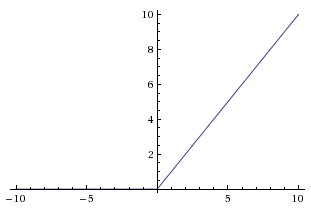
\includegraphics[width=0.7\textwidth]{Pics/relu}\\
                        \small{Rectified Linear Unit (ReLU): $f(x)=max(0,x)$}
                \end{figure}

	\end{columns}

\end{frame}

\begin{frame}
        \frametitle{Neural network architecture}

	Collection of neurons connected in an acyclic graph.\\
	Last output layer represents class scores.

        \begin{columns}
                \column{0.5\textwidth}
                \begin{figure}
                        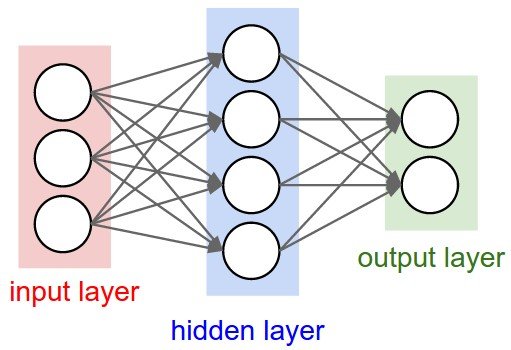
\includegraphics[width=0.7\textwidth]{Pics/neural_net}\\
                        \small{A 2-layer Neural Network}\\
			Size: \pause 4 + 2 = 6 neurons, [3 x 4] + [4 x 2] = 20 weights and 4 + 2 = 6 biases, for a total of 26 learnable parameters.
                \end{figure}
                \column{0.5\textwidth}
                \begin{figure}
                        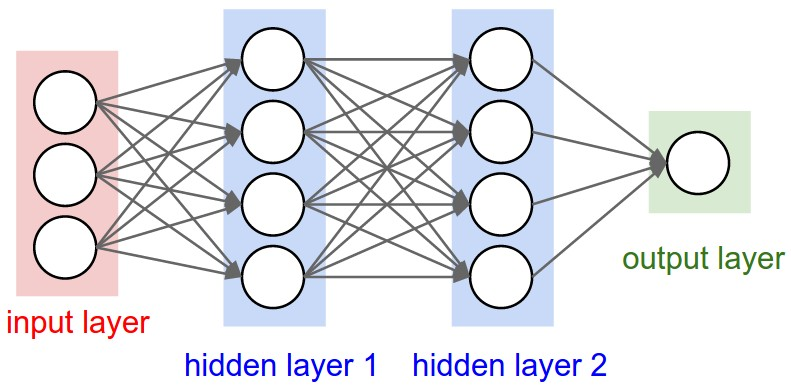
\includegraphics[width=0.7\textwidth]{Pics/neural_net2}\\
                        \small{A 3-layer Neural Network}\\
			Size: \pause 4 + 4 + 1 = 9 neurons, [3 x 4] + [4 x 4] + [4 x 1] = 12 + 16 + 4 = 32 weights and 4 + 4 + 1 = 9 biases, for a total of 41 learnable parameters.
                \end{figure}

        \end{columns}

\end{frame}

\begin{frame}
	\frametitle{Representational power}

	Given any continuous function $f(x)$ and some $\epsilon > 0$, there exists a Neural Network $g(x;W)$ 
	with one hidden layer (with a reasonable choice of non-linearity, e.g. sigmoid) such that for 
	all $x$, $\mid f(x)-g(x) \mid <\epsilon$. 

	\vskip 0.5cm

	In other words, the neural network can approximate any continuous function.

	\vskip 0.5cm

	In practice, more layers work better...

\end{frame}

\begin{frame}
	\frametitle{Setting up the architecture}

	\begin{figure}
        	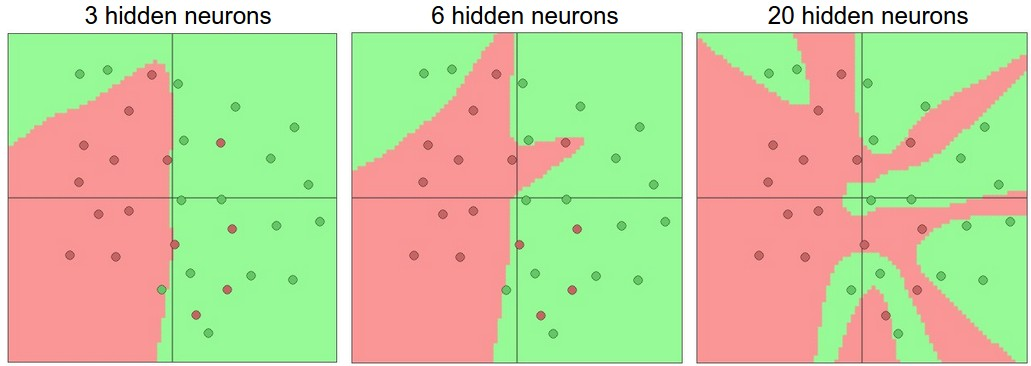
\includegraphics[width=0.8\textwidth]{Pics/layer_sizes}
      	\end{figure}

	Capacity vs. ? \pause Overfitting

	We aim at a better \textbf{generalisation}.

\end{frame}


\begin{frame}
	\frametitle{Setting up the data}

	Data preprocessing:
	\begin{itemize}
		\item mean subtraction
		\item normalisation
		\item PCA and Whitening
	\end{itemize}

\end{frame}


\begin{frame}
        \frametitle{Setting up the model}

        Weights' initialisation:
        \begin{itemize}
                \item all zero
                \item small random numbers
                \item calibrate the variances
		\item sparse
        \end{itemize}

\end{frame}

\begin{frame}
        \frametitle{Setting up the model}

	Regularisation

        \begin{figure}
                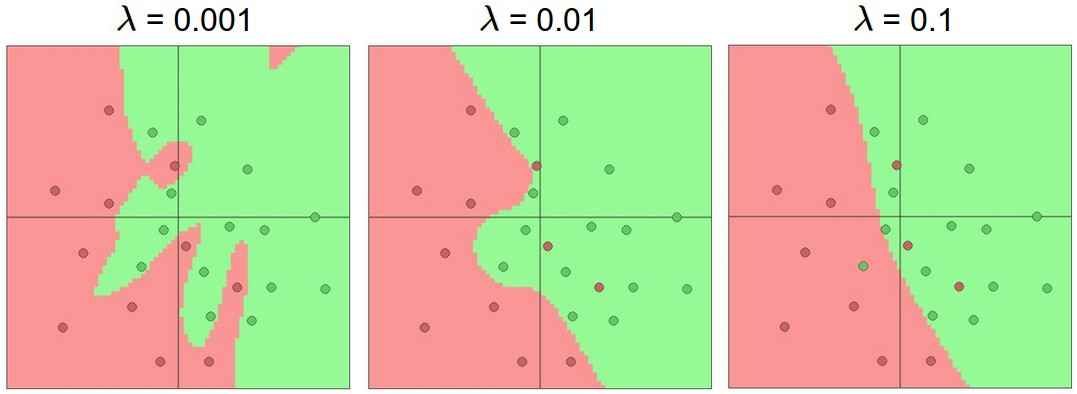
\includegraphics[width=0.8\textwidth]{Pics/reg_strengths}
        \end{figure}

        Options: L2, L1, maxnorm and dropout.

\end{frame}

\begin{frame}
	\frametitle{Dropout}

	\begin{figure}
                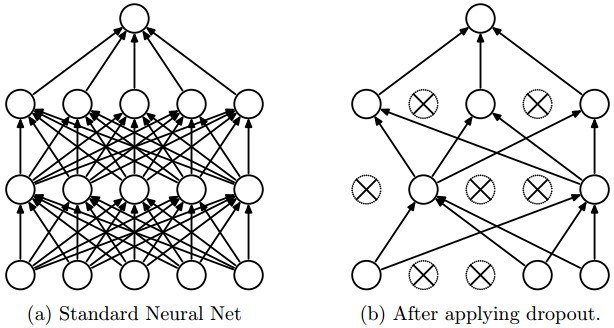
\includegraphics[width=0.8\textwidth]{Pics/dropout}
        \end{figure}

	Dropout can be interpreted as sampling a Neural Network within the full Neural Network, 
	and only updating the parameters of the sampled network based on the input data. 


\end{frame}


\begin{frame}
        \frametitle{Setting up the model}

        Loss functions:
	\begin{itemize}
                \item SVM (hinge loss)
                \item cross-entropy
                \item hierarchical softmax
                \item attribute classification
		\item for regression
        \end{itemize}

\end{frame}

\begin{frame}
	\frametitle{Setting up the learning}

	\begin{columns}
                \column{0.5\textwidth}
                \begin{figure}
                        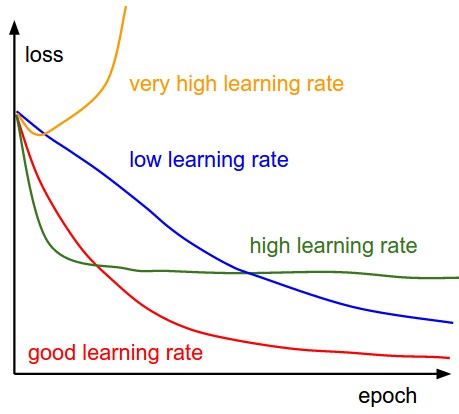
\includegraphics[width=0.8\textwidth]{Pics/learningrates}\\
                        \small{effects of different learning rates}
                \end{figure}
                \column{0.5\textwidth}
                \begin{figure}
                        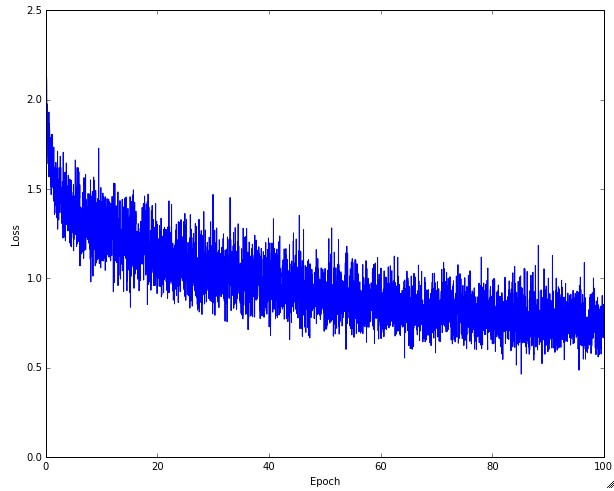
\includegraphics[width=0.8\textwidth]{Pics/loss}\\
                        \small{loss decay}
                \end{figure}

        \end{columns}

\end{frame}

\begin{frame}
        \frametitle{Setting up the learning}

	Training vs. validation accuracy

     	\begin{figure}
     		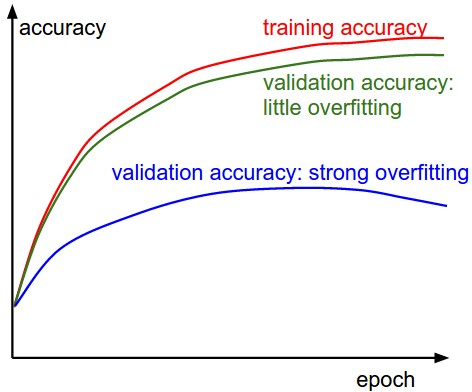
\includegraphics[width=0.5\textwidth]{Pics/accuracies}\\
    	\end{figure}

\end{frame}


\begin{frame}
	\frametitle{Wrap up}

	\begin{itemize}
		\item Neural Networs are made of layers of neurons/units with activation functions
		\item Choice of the architecture: capacity vs overfitting
		\item Preprocessing of the data and choice of hyperparameters for the model and learning
	\end{itemize}

	What about images? Can we use neural networks straight from images? What's the issue?

\end{frame}

















\section{convnets}

\begin{frame}
	\frametitle{Convolutional Neural Networks (CNN)}

	\begin{columns}
       		\column{0.5\textwidth}
      		\begin{figure}
             		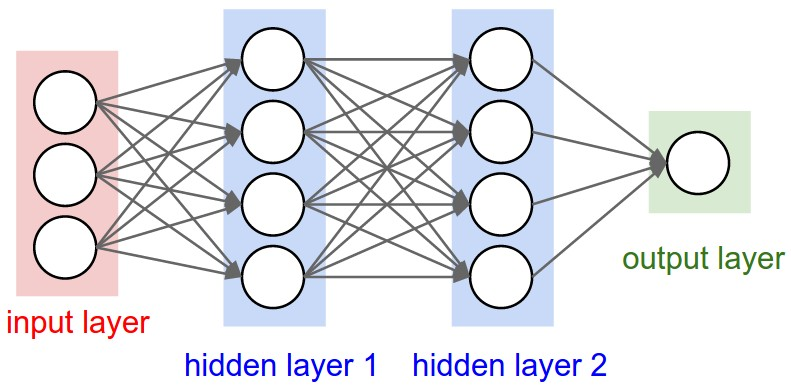
\includegraphics[width=1\textwidth]{Pics/neural_net2}
                \end{figure}
                \column{0.5\textwidth}
                \begin{figure}
                        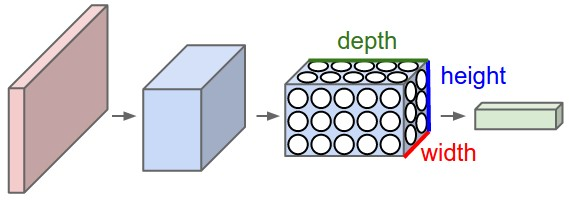
\includegraphics[width=1\textwidth]{Pics/cnn}
                \end{figure}

        \end{columns}

	\vskip 0.5cm

	A CNN arranges its neurons in three dimensions (width, height, depth). 
	Every layer of a CNN transforms the 3D input volume to a 3D output volume of neuron activations.
	Neurons in a layer are connected only to a small region of the layer before it.

\end{frame}


\begin{frame}
	\frametitle{CNN architecture}

	\begin{itemize}
		\item Convolutional Layer
		\item Pooling Layer
		\item Fully-Connected Layer
	\end{itemize}

	We will stack these layers to form a full CNN architecture.

\end{frame}

\begin{frame}
	\frametitle{Convolutional layer}

	\begin{figure}
       		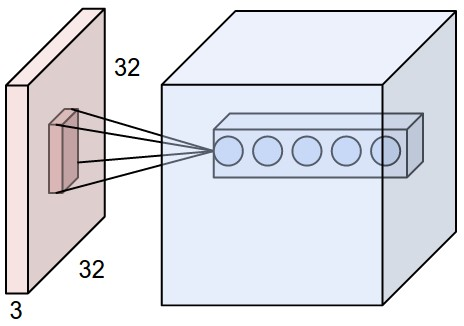
\includegraphics[width=0.4\textwidth]{Pics/depthcol}
      	\end{figure}

	Set of learnable filters which \textit{slides} across the width and height of the input volume.\\
	3 hyper-parameters: depth (nr of filters), stride, zero-padding.

\end{frame}

\begin{frame}
        \frametitle{Convolutional layer}

	\begin{itemize}
		\item Accepts a volume of size $W_1xH_1xD_1$
		\item Requires 4 parameters: number of filters $K$, their size $F$, the stride $S$, the amount of zero padding $P$
		\item Produces a volume of size $W_2xH_2xD_2$ where:
		\begin{itemize}
			\item $W_2 = (W_1 - F +2P)/S+1$
			\item $H_2 = (H_1 - F +2P)/S+1$
			\item $D_2 = K$
		\end{itemize}
	\end{itemize}

	Usually: $F=3$,$S=1$,$P=1$.

	Demo: \url{http://cs231n.github.io/convolutional-networks/}

\end{frame}

\begin{frame}
        \frametitle{Weights in filters}

        \begin{figure}
                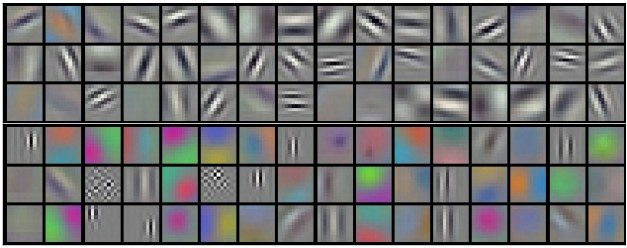
\includegraphics[width=0.9\textwidth]{Pics/weights}\\
		\small{Example filters learned by Krizhevsky et al. Each of the 96 filters shown here is of size [11x11x3], and each one is shared by the 55*55 neurons in one depth slice}
        \end{figure}

\end{frame}


\begin{frame}
        \frametitle{Pooling layer}

        \begin{columns}
                \column{0.5\textwidth}
                \begin{figure}
                        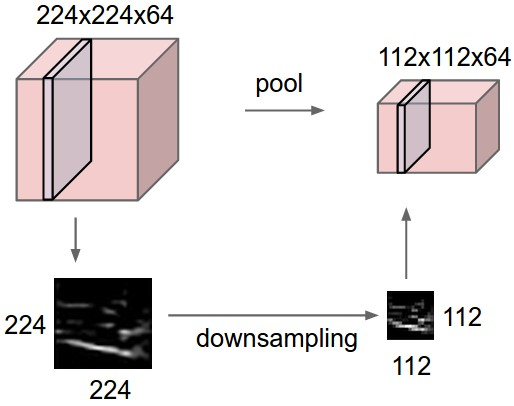
\includegraphics[width=1\textwidth]{Pics/pool}
                \end{figure}
                \column{0.5\textwidth}
                \begin{figure}
                        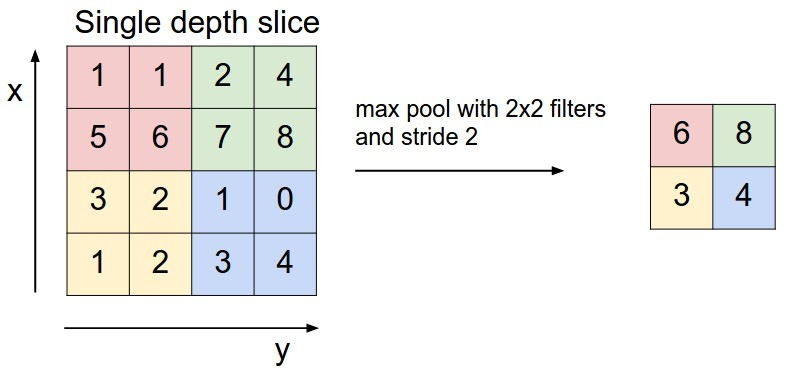
\includegraphics[width=1\textwidth]{Pics/maxpool}
                \end{figure}

        \end{columns}

	\vskip 0.5cm
	Size will influence the proportion of weights retained.

\end{frame}

\begin{frame}
	\frametitle{Layer patterns}

	INPUT $\rightarrow$ [[CONV $\rightarrow$ RELU]*N $\rightarrow$ POOL?]*M $\rightarrow$ [FC $\rightarrow$ 
	RELU]*K $\rightarrow$ FC

	\vskip 1cm

	More examples: \url{http://cs231n.github.io/convolutional-networks/}

\end{frame}

\begin{frame}
	\frametitle{Applications to biological data}

	From various sources:
	\begin{itemize}
		\item -omics (gen-, transcript-, epigen-, prote-, metabol-)
		\item bioimaging (cellular images, ...)
		\item medical images (clinical imaging)
		\item brain/body machine interfaces (ECG, EEG, ...)
	\end{itemize}

\end{frame}

\begin{frame}
        \frametitle{Applications to biological data}

	\begin{figure}
                \includegraphics[width=0.6\textwidth]{Pics/biology.png}
        \end{figure}

\end{frame}

\begin{frame}
	\frametitle{Omics}

	Mining DNA/RNA sequence data to:
	\begin{itemize}
		\item identify splicing junction
		\item classify somatic point mutation-based cancer
		\item predict DNA- and RNA-binding motifs
		\item relate disease-associated variants to gene expression
		\item estimate DNA methylation patterns
		\item ...
	\end{itemize}

\end{frame}

\begin{frame}
	\frametitle{Splice junctions}

	\vskip 0.3cm
	Deep neural networs outperform other methods.

	\begin{figure}
                \includegraphics[width=0.45\textwidth]{Pics/splice.png}
        \end{figure}

\end{frame}

\begin{frame}
	\frametitle{Open issues}

	\begin{itemize}
		\item theory of deep learning is not completely understood making outcomes difficult to interpret
		\item susceptible to misclassification and overclassification
		\item uncertainty in building architectures
		\item bootstrapping not possible
	\end{itemize}

\end{frame}

\begin{frame}
        \frametitle{Future perspectives}

        \begin{itemize}
		\item improving theoretical foundations on the basis of experimental data
		\item assessment of model's computational complexity and learning efficiency
		\item novel data visualization tools
		\item in biology: reduce data redundancy and extract novel information
		\item \textit{ad hoc} computational infrastructures
	\end{itemize}

\end{frame}

\begin{frame}
        \frametitle{Wrap up}

        \begin{itemize}
                \item CNN arranges its neurons in three dimensions
                \item Different type of layers (convolution, pooling, ...)
                \item Weights in filters are learned
		\item Promising applications to biological data.
        \end{itemize}

\end{frame}











\section{keras}

\begin{frame}
        \frametitle{TensorFlow}

        \begin{figure}
        	\includegraphics[width=0.5\textwidth]{Pics/tensorflow.png}
        \end{figure}

	easy and intuitive way to do ML

\end{frame}

\begin{frame}
        \frametitle{TensorFlow}

        \begin{figure}
                \includegraphics[width=0.5\textwidth]{Pics/tf_code.png}
        \end{figure}

	concept-heavy but code-light

	many parameters, but only few are important to adjust

\end{frame}

\begin{frame}
        \frametitle{TensorFlow}

        \begin{figure}
                \includegraphics[width=0.9\textwidth]{Pics/tf_api.png}
        \end{figure}

\end{frame}

\begin{frame}
        \frametitle{Low-level APIs}

	What is a tensor?

        \begin{figure}
                \includegraphics[width=0.7\textwidth]{Pics/tensor.png}
        \end{figure}

	\begin{figure}
                \includegraphics[width=0.4\textwidth]{Pics/graph.png}
        \end{figure}

\end{frame}

\begin{frame}
	\frametitle{Examples of data tensors}

	\begin{itemize}
		\item vector data: 2D tensors of shape \texttt{(samples, features)}
		\item timeseries or sequence data: 3D tensors of shape \texttt{(samples, timesteps, features)}
		\item images: 4D tensors of shape \texttt{(samples, height, width, channels)}
		\item video: 5D tensors of shape \texttt{(samples, frames, height, width, channels)}
	\end{itemize}

	\small{The first axis is the sample or batch dimension.}

\end{frame}

\begin{frame}
	\frametitle{Image data}

	\begin{figure}
                \includegraphics[width=0.6\textwidth]{Pics/image.jpg}
        \end{figure}

	\small{A batch of 128 colour images can be stored in a 4D tensor with shape \texttt{(128,256,256,3)}}

\end{frame}

\begin{frame}
        \frametitle{Anatomy of a neural network}

        \begin{figure}
                \includegraphics[width=0.5\textwidth]{Pics/nn_scheme.jpg}
        \end{figure}

\end{frame}


\begin{frame}
	\frametitle{Build your first neural network}

	\begin{enumerate}
		\item collect and preprocessing a dataset: most of the actual work
		\pause
		\item build your model: few lines of code
		\pause
		\item train: one line of code
		\pause
		\item evaluate: one line of code
		\pause
		\item predict: one line of code
	\end{enumerate}

	\bigskip
	\tiny{source: Get started with TensorFlow's High-Level APIs (Google I/O '18)}

\end{frame}

\begin{frame}
	\frametitle{Step 1: collect a dataset}

	Import the data and spend a lot of time asking questions on: rank, shape, number of objects, printing, format, data type, ...: very basic questions!


	 \begin{figure}
                \includegraphics[width=0.6\textwidth]{Pics/tf_1.png}
        \end{figure}
	
\end{frame}

\begin{frame}
        \frametitle{Step 1: collect a dataset}

         \begin{figure}
                \includegraphics[width=0.4\textwidth]{Pics/fashion-mnist.png}
        \end{figure}

	\small{70,000 28x28 grayscale images in 10 categories of clothing articles}

\end{frame}

\begin{frame}
        \frametitle{Step 1: collect a dataset}

         \begin{figure}
                \includegraphics[width=0.9\textwidth]{Pics/tf_2.png}
        \end{figure}

	 \begin{figure}
                \includegraphics[width=0.9\textwidth]{Pics/tf_3.png}
        \end{figure}

\end{frame}

\begin{frame}
        \frametitle{Step 2: build a model}

	\begin{figure}
                \includegraphics[width=0.9\textwidth]{Pics/nn_google.png}
        \end{figure}

\end{frame}

\begin{frame}
        \frametitle{Step 2: build a model}

	\begin{itemize}

	\item start simple! do not overlearn the training set.

	\item define loss function

	\item define optimization (important but defaults are good)

	\end{itemize}

	\begin{figure}
                \includegraphics[width=0.9\textwidth]{Pics/compile.png}
        \end{figure}

	\small
	When you choose a network topology, you constrain your space of possibilities (hypothesis space) 
	to a specific series of tensor operations, mapping input data to output data.

\end{frame}

\begin{frame}
        \frametitle{Step 3: train the model}

	 \begin{figure}
                \includegraphics[width=0.9\textwidth]{Pics/train.png}
        \end{figure}

	Only "epochs" (and "batch size") matter here.

\end{frame}

\begin{frame}
	\frametitle{Step 4: evaluate}

	\begin{figure}
                \includegraphics[width=0.9\textwidth]{Pics/evaluate.png}
        \end{figure}

\end{frame}

\begin{frame}
	\frametitle{Step 5: predict}

	\begin{figure}
                \includegraphics[width=0.9\textwidth]{Pics/predict.png}
        \end{figure}

	\url{https://www.tensorflow.org/tutorials/keras/basic_classification}

\end{frame}

\begin{frame}
        \frametitle{Keras}

         \begin{figure}
                \includegraphics[width=0.6\textwidth]{Pics/keras.png}
        \end{figure}

	"Keras is a high-level neural networks API, written in Python and capable of running on 
	top of TensorFlow, CNTK, or Theano."

\end{frame}

\begin{frame}
        \frametitle{Keras}

         \begin{figure}
                \includegraphics[width=0.5\textwidth]{Pics/keras2.jpg}
        \end{figure}

\end{frame}




\begin{frame}
        \frametitle{Intended Learning Outcomes}

        At the end of this session, you are now be able to:
        \begin{itemize}
                \item Describe the three key components of a classifier: score function, loss function, optimisation
                \item Identify the elements of a neural networks, including neurons and hyper-parameters
                \item Illustrate the specific layers in a neural network for visual recognition
                \item Appreciate the use of deep learning to solve biological problems
                \item Demonstrate how to implement, train and evaluate a deep neural network in \texttt{python}
        \end{itemize}

\end{frame}


\section{Practical}

\begin{frame}
        \frametitle{IUCN Red List of Threatened Species}

        \begin{columns}
                \column{0.5\textwidth}
                LC: least concern
                \begin{figure}
                        \includegraphics[height=0.2\textheight]{Pics/LC}
                \end{figure}
                VU: vulnerable
                \begin{figure}
                        \includegraphics[height=0.2\textheight]{Pics/VU}
                \end{figure}
                \column{0.5\textwidth}
                EN: endangered
                \begin{figure}
                        \includegraphics[height=0.2\textheight]{Pics/EN}
                \end{figure}
                CR: critically endangered
                \begin{figure}
                        \includegraphics[height=0.2\textheight]{Pics/CR}
                \end{figure}
        \end{columns}

\end{frame}


\begin{frame}
        \frametitle{Population genetics}

        \begin{figure}
        	\includegraphics[width=1\textwidth]{Pics/sara.png}
        \end{figure}

\end{frame}

\begin{frame}
	\frametitle{Population genetics}
	
	\begin{figure}
		\centering
		\includegraphics[height=0.8\textheight]{Pics/simulations.png}
	\end{figure}

\end{frame}

\begin{frame}{Genomic data}

	\begin{figure}
    		\includegraphics[width=0.4\textwidth]{Pics/example.png}
	\end{figure}

	haplotypes/individuals on rows, genomic positions on columns

\end{frame}

\begin{frame}{CNN applied to population genomic data}

    \begin{figure}
        \includegraphics[width=0.9\textwidth]{Pics/flagel.png}
        \end{figure}

\end{frame}



















\begin{frame}
        \frametitle{Who is the \textit{deepest learner}?}

        \centering{It's a competition!}

        \begin{columns}
                \column{0.6\textwidth}
                The challenge: predict whether a species is endangered, vulnerable or of least
                concern from genomic data.
                \column{0.4\textwidth}
                \begin{figure}
                        \includegraphics[width=0.8\textwidth]{Pics/ursus.jpg} \\
                        \tiny{\textit{Ursus arctos marsicanus}}
                \end{figure}
        \end{columns}

        \vskip 1cm

        The score to beat: 75\% by me.

        The prize: a free drink at the pub.

\end{frame}


\begin{frame}
	\frametitle{Well done!}

	\vskip 0.2cm
	\small{You are all data scientists* now!}

	\begin{figure}
                \includegraphics[width=0.35\textwidth]{Pics/machine_learning.png}
        \end{figure}

	\vskip 0.5cm
	\centering
	\footnotesize{*data science: statistics done by non-statisticians}

\end{frame}

\end{document}

